\section{Devices}

When describing his vision for Ubiquitous Computing, Weiser draws a parallel to the evolution of the electric engine:

\begin{quote}
    How do technologies disappear into the background? The vanishing of electric motors may serve as an instructive example.
    At the turn of the century, a typical workshop or factory contained a single engine that drove dozens or hundreds of
    different machines through a system of shafts and pulleys. Cheap, small, efficient electric motors made it possible first
    to give each tool its own source of motive force, then to put many motors into a single machine.\cite{weiser91}
\end{quote}

Electric engines are in some ways like computers, but in other ways entirely unlike them. Both have had a development where
they have shrunk dramatically in size. Unlike electric engines, however, computers perform more than one task. Comparing electric
engines to computers is like comparing processors to machines - one is nothing more than a component of something bigger.

A \emph{device} is an entity consisting of several components (processors, sensors, NFC chips, and more) that performs more
than one task. That is, unlike motion sensors, which only sense motion, a device is a collection of functionality in a single
computer. Devices are, in their very nature, anti-ubiquitous computers, as they demand attention, rather than become
invisible,\footnote{Weiser writes that "multimedia tries to grab attention, the opposite of the ubiquitous computing ideal of
invisibility"\cite{weiser93}} and are in no way single-purpose.

Examples of devices are easy to find: laptops, personal computers, smartphones, and tablets. All of these perform the same, common
tasks (multimedia -- watching and reading; office work -- timekeeping, writing; etc.). They are the epitome of redundancy, and yet
they are very popular.\footnote{Cisco projects 3 devices per capita in the world by 2017.\cite{cisco}}

\subsection{Co-existence}

Weiser does not claim that Ubiquitous Computing must be the only kind of computing present, for the ubiquitous state to be reached.
Rather, it will coexist with Personal Computing for a while, until it eventually becomes more popular and pushes Personal Computing
out of the picture, he argues (see Figure \ref{fig:trends-graph}).

\begin{figure}[ht]
	\centering
	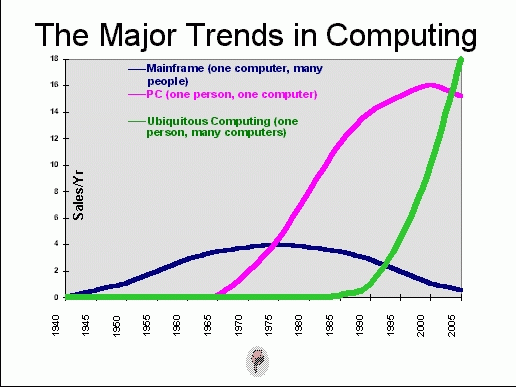
\includegraphics[width=0.75\textwidth]{multipurpose/trends-graph}
	\caption{Trends in computing, according to Weiser, depicting Ubiquitous Computing overtaking Personal Computing in sales around
		2004. This prediction was orignally made in 1996.\cite{weisernomadic}}
	\label{fig:trends-graph}
\end{figure}

Devices are a modern incarnation of Personal Computing, allowing personal computers to be accessed in more places. The over-simplification
used in Weiser's graph, indicating that only Ubiquitous Computing can have several computers for one person, may cause confusion. Devices
are, however, in no way ubiquitous. Each of the most commonly used devices performs each of the most used tasks. As explained above, devices
are not single-purpose, nor are they invisible.

We have, indeed, seen Ubiquitous Computing grow in popularity, with sensors, NFC chips, and the likes becoming increasingly used. But
while this was a trend for some time, we are now seeing a competing trend take over some of the fields that were dominated by ubiquity:
the trend of devices.

Wearable technology seems like a natural extension of Ubiquitous Computing, as wearable technology has a natural tendency to blend with
the user, and -- as a result of this -- become invisibe. A tiny device measures your pulse when you go running, and another offers
to track your location when walking.\footnote{Sources for old devices that did this, and only this, missing.} But despite there still
being launched truly ubiquitous, single-purpose, invisible, wearable technology (such as FitBit, a wearable fitness tracker\footnote{See
this: http://www.fitbit.com.}) there is a conflicting tendency towards gathering up all the functionality in devices, such as Apple's
upcoming iWatch, a device worn on your wrist, which could indeed track things such as pulse and location.\footnote{Source on iWatch!}

The tendency seems to be that new \emph{things to measure} and \emph{ways to measure} start out truly as ubiquitous computers, that do
nothing more than measure and communicate, until the idea becomes popular enough to be scooped up in a very un-ubiquitous device.

Note: Mention the project that is trying to make smartphones replace travel cards, payment cards, access cards.

Google Glass,\footnote{Source} a recent, high-profile piece of wearable technology is very much a device, and, together with the iWatch,
goes to show the tendency of the device idea moving into fields traditionally held by Ubiquitous Computing. It is not the case that all
Ubiquitous Computing is disappearing, but rather that it is only desirable for a few, specific areas. Sensors tracking movement (and, for
example, turn on patio lights) are not going to be integrated into devices, and it is indeed an advantage that these sensors are out of sight.

For the vast majority of features, however, devices seem to dominate, and Weiser's quote from 1991 is as true today as it was in its
time: "Today's multimedia machine makes the computer screen into a demanding focus of attention rather than allowing it to fade into the
background."\cite{weiser91} I would argue that this happens because the end-user wants to be in control of the technology.

\subsection{Choice}

The uprising of devices results in the computers being less \emph{inescapably} everywhere and more \emph{accessibly} everywhere. In the words
of a popular fast-food chain, "Choice is King"\footnote{Burger King lol.}.

We want to be able to take things with us. We want to be able to put things down. This is what makes ubicomp undesirable.

\begin{quote}
    Doors open only to the right badge wearer, rooms greet people by name, telephone calls can be automatically forwarded to wherever the recipient may be, receptionists actually know where people are, computer terminals retrieve the preferences of whoever is sitting at them and appointment diaries write themselves. The automatic diary shows how such a simple task as knowing where people are can yield complex dividends\cite{weiser91}
\end{quote}

We might get several devices (one person has laptop, tablet, smartphone) but each device does everything.

We lose the single-purpose. We lose the invisible (they draw attention). We lose the everywhere (they are in specific places
so we can put them away). To some extent we lose the many, as we seem to stagnate around 3 devices per person.\footnote{Cisco
predicts that there will, in 2017 be "nearly three networked devices per capita". This includes business devices, so 3 is a
high number for a long time.\cite{cisco} Of course, there are also other devices, such as ovens and microwaves. This ends up
with a count of around 30 in a normal household. Well below 100. --- A different survey counts a maxiumum (Switzerland) of
0,86 devices per person in 2005. This is still well within my prediction.\cite{nationmaster}} The only thing we keep is the small.

Security/privacy concerns. With the recent NSA scandal and the likes, people might want to be able to escape computers.
On the other hand, people are willingly using Google, etc., letting it track them. There seems to be a split. Some people
willingly and intentionally share \emph{everything}, some share a limited number of things, and a tiny group shares nothing
at all, making an effort to escape the surveilance.\footnote{Soruces on this?!} This choice would be entirely impossible
with true ubicomp.

---

Note: Find a graph of sales/data on it, and show that devices are GROWING (also supported by cisco),